\section{Технический проект}
\subsection{Общая характеристика организации решения задачи}

Необходимо спроектировать и разработать сайт, который должен способствовать успешной продаже курсов по программированию.

Интернет-сайт представляет собой набор взаимосвязанных электронных страниц, которые сгруппированы по разделам, содержащие текстовую, графическую, а также мультимедийную информацию (изображения и пр.). Сайт располагается в Интернете по определенному адресу – доменному имени сайта в виде www.имя\_сайта.ru. Каждая страница web-сайта – это текстовый документ, написанный на языке программирования (HTML, CSS, JavaScript и т.д.).

\subsection{Обоснование выбора технологии проектирования}

На сегодняшний день информационный рынок, поставляющий программные решения в выбранной сфере, предлагает множество продуктов, позволяющих достигнуть поставленной цели – разработки web-сайта.

\subsubsection{Описание используемых технологий и языков программирования}

В процессе разработки web-сайта используются программные средства и языки программирования. Каждое программное средство и каждый язык программирования применяется для круга задач, при решении которых они необходимы.

\subsubsection{Язык программирования Python}

Python – высокоуровневый язык программирования общего назначения с динамической строгой типизацией и автоматическим управлением памятью, ориентированный на повышение производительности разработчика, читаемости кода и его качества, а также на обеспечение переносимости написанных на нём программ. Использование Python позволило мне легко и эффективно разрабатывать серверную часть проекта, обеспечивая стабильную работу и высокую производительность.

\subsubsection{Язык программирования HTML}

Для разработки клиентской части проекта и отображения информации для пользователей, я использовал язык разметки HTML (HyperText Markup Language). HTML - это стандартный язык, используемый для создания веб-страниц, и он играет ключевую роль во взаимодействии пользователей с моим сервером.

Вот некоторые из основных плюсов HTML:
Простота и доступность: HTML - это язык разметки, который легко учить и использовать. 

Универсальность: HTML поддерживается практически всеми браузерами и устройствами, что позволяет создавать веб-страницы, доступные для широкой аудитории.

Семантика: HTML предоставляет разнообразные элементы и атрибуты для описания структуры и содержания веб-страницы. 

Версионная совместимость: HTML постоянно развивается, и новые версии (например, HTML5) включают в себя новые возможности и элементы. Это обеспечивает совместимость с более ранними версиями HTML и позволяет использовать современные функции.


\subsubsection{Язык программирования JavaScript}

JavaScript является ключевым языком для разработки клиентской части веб-приложений. Вот почему я выбрал JavaScript:

Интерактивность и динамичность: JavaScript позволяет создавать динамичные и интерактивные пользовательские интерфейсы. Это включает в себя асинхронное взаимодействие с сервером и изменение содержимого страницы без ее перезагрузки.

Широкая поддержка в браузерах: JavaScript поддерживается практически всеми современными браузерами, что обеспечивает высокую степень переносимости кода.

Возможности асинхронного программирования: JavaScript поддерживает асинхронный код, что особенно важно при работе с операциями ввода/вывода, такими как запросы к серверу или обработка событий.

Быстрое выполнение в браузере: JIT-компиляция в современных браузерах позволяет JavaScript выполняться достаточно быстро, что особенно важно для обеспечения быстрого отклика интерфейса.

\subsubsection{Язык разметки CSS}

CSS используется для оформления и стилизации веб-страниц. Вот почему я выбрал CSS:

Отделение структуры и стиля: CSS позволяет разделять структуру HTML и ее визуальное оформление, что упрощает обслуживание и обновление кода.

Множество возможностей стилизации: CSS предоставляет широкий набор возможностей для стилизации, включая цвета, шрифты, размеры, позиционирование и анимации.

\subsection{Диаграмма взаимодействия и схема обмена данными между представлениями}

Диаграмма взаимодействия описывает особенности физического представления разрабатываемой системы. Она позволяет определить архитектуру системы, установив зависимости между программными представлениями, в роли которых может выступать как исходный, так и исполняемый код. Основными графическими элементами диаграммы взаимодействия являются представлениями, интерфейсы, а также зависимости между ними. На рисунке \ref{comp:image} изображена диаграмма представлениями для проектируемой системы. Она включает в себя сервер с операционной системой, на которой установлена система управления содержимым, включающая в себя базу данных и интерфейс. Помимо этого на диаграмме изображен клиентский компьютер с операционной системой, на которой установлен браузер.

\begin{figure}[ht]
\center{\includegraphics[width=1\linewidth]{comp}}
\caption{Диаграмма компонентов}
\label{comp:image}
\end{figure}

Любое представление должно быть вызвано в сценарии страницы web-сайта. Web-страница передает данные представления в момент вызова последнего.

На рисунке \ref{представления:image} представлена схема обмена данными между сценариями представления при вызове представления на странице сайта.

\begin{figure}[ht]
\center{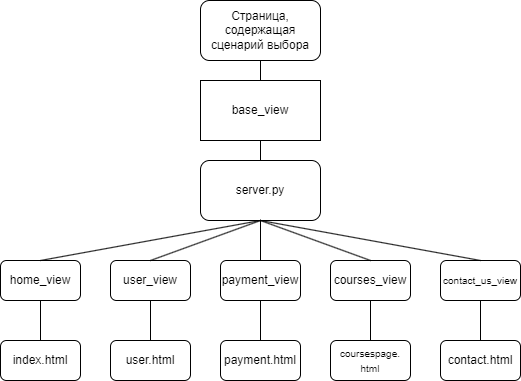
\includegraphics[width=1\linewidth]{представления}}
\caption{Диаграмма представления}
\label{представления:image}
\end{figure}

В файле server.py написан код, который представляет собой простое веб-приложение на Python, использующее фреймворк WSGI (Web Server Gateway Interface).

Здесь импортируются различные библиотеки, классы и функции, которые используются в приложении, такие как CGI, Waitress для веб-сервера, различные представления (views) и функции для работы с файлами и базой данных. Словарь urls соотносит URL-пути с соответствующими представлениями. Когда приходит запрос, код использует этот словарь для определения, какой обработчик использовать для данного URL. Основная функция app обрабатывает POST запрос для загрузки файла, извлекает данные из формы, вставляет изображение в БД и возвращает ответ в формате JSON. Обработка GET запроса происходит с логики определения и вызова соответствующего представления и логики для обработки статических файлов, определение MIME-типа и кодировки для ответа, а также установка заголовков ответа и возврат данных в ответе.

\subsection{Диаграмма размещения}

Диаграмма размещения (рис.~\ref{place:image}) отражает физические взаимосвязи между методами и представлениями.

\vspace{-8mm} % чтобы убрать пустую строку, которая осталась после переноса рисунка на следующую страницу
\begin{figure}[ht]
\center{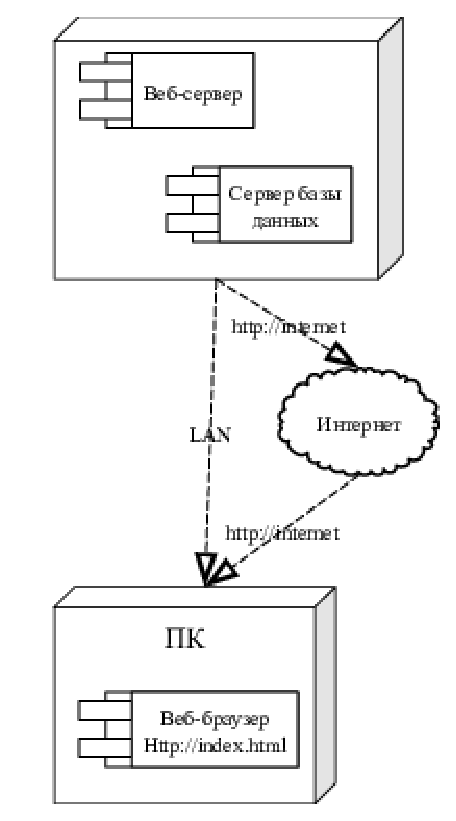
\includegraphics[width=0.57\linewidth]{place}}
\caption{Диаграмма размещения}
\label{place:image}
\end{figure}

Она является хорошим средством для показа маршрутов перемещения объектов и компонентов в распределенной системе.

\subsection{Содержание информационных блоков. Основные сущности}

Проанализировав требования, можно выделить две основных сущности:
\begin{itemize}
	\item "<Пользователь">;
	\item "<Покупка курса">;
\end{itemize}

В состав сущности "<Пользователь"> можно включить атрибуты, представленные в таблице 3.1.

\begin{xltabular}{\textwidth}{|l|l|p{1.7cm}|X|}
	\caption{Атрибуты сущности "<Пользователь">\label{news:table}}\\ \hline
	\centrow Поле & \centrow Тип & \centrow Обяза\-тельное & \centrow Описание \\ \hline
	\thead{1} & \thead{2} & \centrow 3 & \centrow 4 \\ \hline
	\endfirsthead
	\thead{1} & \thead{2} & \centrow 3 & \centrow 4 \\ \hline
	\finishhead
	id & ObjectId & true & Уникальный идентификатор \\ \hline 
	login & String & true & Логин \\ \hline 
	pass & String & true & Пароль \\ \hline 
\end{xltabular}

В состав сущности "<Покупка курса"> можно включить атрибуты, представленные в таблице 3.2.

\begin{xltabular}{\textwidth}{|l|l|p{1.7cm}|X|}
	\caption{Атрибуты сущности "<Покупка курса">\label{news:table}}\\ \hline
	\centrow Поле & \centrow Тип & \centrow Обяза\-тельное & \centrow Описание \\ \hline
	\thead{1} & \thead{2} & \centrow 3 & \centrow 4 \\ \hline
	\endfirsthead
	\thead{1} & \thead{2} & \centrow 3 & \centrow 4 \\ \hline
	\finishhead
	id & ObjectId & true & Уникальный идентификатор \\ \hline 
	name & String & true & Название курса \\ \hline 
	cost & Integer & true & Цена курса \\ \hline 
	description & String & true & Уровень сложности \\ \hline 
	about & String & true & Описание курса \\ \hline
	image & Longblob & true & Фото \\ \hline 
\end{xltabular}